\chapter{Lancio della moneta e Hard Core Predicate}
\label{chapter8}

Supponiamo di avere Alice e Bob che vogliono lanciare una moneta in rete. Vogliamo costruire un protocollo che sia simile a quello che si ha quando la moneta viene lanciato in presenza. Si potrebbe fare in modo che uno dei due lanci la moneta e poi comunichi il risultato all'altro. Questa soluzione non va bene in quanto chi lancia la moneta può sceglierne arbitrariamente il valore, senza che l'altro agente abbia modo di verificare l'autenticità del valore ricevuto. Non è possibile verificare se la moneta lanciato sia equa.

Possiamo quindi far lanciare una moneta ad entrambi e poi far loro scambiare i risultati. Supponiamo che il risultato sia $0$ quando i valori delle due monete sono diversi e $1$ quando sono uguali. Se almeno uno dei due agenti lancia un moneta equa, la probabilità che il risultato finale sia $0$ è $1/2$. Anche questo soluzione è vulnerabile. Bob potrebbe fingere di spedire il suo risultato e attendere il messaggio di Alice, per poi forgiare di conseguenza il suo messaggio e indurre il risultato che vuole, fingendo un ritardo sulla rete. 

Possiamo appoggiarci ad una terza parte, ma questa soluzione sposta solo il problema della fiducia dai due attori originali ad un altro.\\

\noindent Il nostro obiettivo è costruire un lancio della moneta sicuro che coinvolga solo i due attori iniziali. Supponiamo che $coin_A$ sia una variabile di Alice che dice qual è il risultato finale del lancio della moneta e che $coin_B$ sia una variabile di Bob che dice lo stesso risultato. 

Vogliamo quindi un protocollo tale per cui, alla fine:
\begin{align*}
    coin_A = coin_B \land Pr[coin_A = 0] = \frac{1}{2}
\end{align*}

\noindent Questo può avvenire solo se $A$ e $B$ seguono correttamente il protocollo (sono onesti). In caso contrario si possono verificare tre casi:
\begin{itemize}
    \item Se $A$ è onesto e $B$ è disonesto, allora dobbiamo far si che
    \begin{align*}
        \left| Pr[coin_A = 0] - \frac{1}{2}\right| < k^{-c}
    \end{align*}
     \item Se $B$ è onesto e $A$ è disonesto, allora dobbiamo far si che
    \begin{align*}
        \left| Pr[coin_B = 0] - \frac{1}{2}\right| < k^{-c}
    \end{align*}
    \item Se $A$ e $B$ sono disonesti, non facciamo nulla (non c'è nessuna parte onesta da tutelare).
\end{itemize}

\noindent Come facciamo ad implementare un protocollo del genere?

\section{Lancio di moneta nel pozzo}
Alice: 
\begin{itemize}
    \item Sceglie a caso due numeri primi $p, q$ e calcola $n=pq$; 
    \item Calcola $z \in_R Z_n^*$ con simbolo di Jacobi $\left( \frac{z}{n}\right)=1$;
    \item Invia $n, z$ a Bob.
\end{itemize}

\noindent Bob:
\begin{itemize}
    \item Sceglie $b \in_R \{0, 1\}$;
    \item Invia $b$ a Alice.
\end{itemize}

\noindent Alice 
\begin{itemize}
    \item Invia $p, q$ a Bob.
\end{itemize}

Risultato
Il risultato del lancio della moneta è dato dal seguente calcolo:
\begin{align*}
    b \oplus is\_square(z)
\end{align*}

\noindent Alice lancia la moneta scegliendo a caso un quadrato o un non quadrato in $Z_n^*$. Infatti scegliendo uniformemente un numero in $Z_n^*$ con simbolo di Jacobi $1$, stiamo scegliendo un quadrato con probabilità $1/2$ o un non quadrato con probabilità $1/2$. Bob sceglie anche lui un bit a caso, che assegna a $b$. 
Quando Alice invia a Bob $z$, Bob non ha alcun modo di vedere il valore scelto da Alice, in quanto per farlo, non conoscendo ancora $p$ e $q$, dovrebbe risolvere il problema del residuo quadratico. Quindi quando Bob invia il suo lancio, il valore non è stato in alcun modo scelto in funzione del bit scelto da Alice. Tramite lo XOR tra i due lanci, scopriamo se i risultati sono uguali oppure no.

Poiché l'ordine dei messaggi e quando inviarli è deciso dal protocollo, la vulnerabilità del messaggio inviato in ritardo è risolta. Ma questo protocollo effettivamente funziona?

Questo protocollo è un'istanza del sistema dove Alice e Bob lanciano indipendentemente una moneta, si scambiano il risultato e il risultato è $0$ allora le due monete sono uguali o $1$ se sono diverse. Il vantaggio di questo protocollo è che se almeno uno dei due lancia la moneta in maniera equa, il risultato è equo.
Vediamo se l'algoritmo funziona rispetto ai vari casi che si possono verificare:
\begin{itemize}
    \item Se Alice e Bob sono onesti, allora $z$ è stato campionato secondo una misura casuale e quindi è un quadrato con probabilità $1/2$ o un non quadrato con probabilità $1/2$. Il valore $b$ vale $0$ con probabilità $1/2$ o $1$ con probabilità $1/2$. Tutti conoscono $p, q, z, n, b$ e possono calcolare il risultato. Sia $coin_A$ sia $coin_B$ avranno lo stesso risultato e
    \begin{align*}
        Pr[coin_A = 0] = \frac{1}{2}
    \end{align*}
    \item Se Bob è disonesto, lo può fare in due modi:
    \begin{enumerate}
        \item Può provare a calcolare $b$ in modo non casuale, usando una distribuzione diversa (es: $b=0$ con probabilità $3/4$ e $b=1$ con probabilità $1/4$). Fintanto che Bob calcola, nel modo che vuole, $b$ in modo indipendente dal valore di $z$, il valore scelto sarà sempre uguale alla quadraticità di $z$ con probabilità $1/2$, in quanto lo XOR tra un bit completamente casuale e un bit calcolato in modo non casuale ma indipendente dall'altro elemento dell'operazione resta comunque casuale;
        \item Può calcolare $b$ in funzione di $z$. Ma questo è equivalente a indovinare la quadraticità di $z$, e quindi ad usare un algoritmo che è in grado di calcolare la quadraticità di $z$. Questo algoritmo dovrebbe essere in grado di stabilire se un numero è un quadrato con un vantaggio polinomiale rispetto a $1/2$. A questo punto l'eventuale attacco di Bob diventerebbe un algoritmo per la risoluzione del problema del residuo quadratico, che consideriamo difficile. 
    
        Abbiamo quindi dimostrato che se questo protocollo fosse attaccabile da Bob, allora il problema che sta alla base sarebbe facile, cosa non possibile in quanto è un problema difficile.
    \end{enumerate}

    \item Se Alice è disonesta, lo può fare in più modi:
    \begin{enumerate}
        \item Può calcolare $p, q$ \textbf{non} primi, ma Bob se ne accorgerebbe quando li riceve al termine del protocollo. In questo caso possiamo considerare nullo il risultato e far rilanciare una moneta a Bob;
        \item Può scegliere $z$ non uniformemente tra gli elementi con simbolo di Jacobi $1$. Se Alice sceglie un elemento con simbolo di Jacobi $-1$, Bob se ne accorgerebbe comunque alla fine. Potrebbe quindi scegliere $z$ con un algoritmo diversa da quello casuale. $Bob$, quando riceve $z$, non ha modo di accorgersi che Alice ha scelto $z$ in maniera non conforme. Ma Bob sceglie comunque il suo bit in modo casuale, rendendo comunque lo XOR casuale;
        \item Può inviare $p, q$ sbagliati, ma Bob se ne accorgerebbe e quindi potrebbe lanciare una sua moneta per decidere il risultato. Ma se invece non li inviasse proprio a Bob? 
        
        Dire che Bob lancia la sua moneta crea una grandissimo svantaggio nei suoi confronti. Alice, una volta ricevuto $b$ da Bob potrebbe rifiutarsi di inviare il messaggio finale, influenzando la probabilità con cui Bob ottiene, ad esempio $0$. Come fa ad alterare la probabilità? Dopo il secondo messaggio alice conosce $coin_A$, in quanto può calcolare lo XOR, ma Bob non conosce ancora $coin_B$.
        Supponiamo che il risultato del lancio della moneta decida chi sale sull'elicottero funzionante e che sull'elicottero manomesso. Se $coin_A$ dice ad Alice di salire sull'elicottero che cade, e quindi le è sfavorevole, allora Alice può non spedire il terzo messaggio. Bob allora lancia la propria moneta, che con probabilità $1/2$ sarà favorevole a lui e con probabilità $1/2$ sarà favorevole ad Alice. 
        Supponendo che $coin_B = 0$ sia il risultato favorevole ad Alice, la probabilità di ottenerlo diventa
        \begin{align*}
            Pr[coin_B = 0] &= Pr[coin_A = 0] + Pr[coin_A = 1] \cdot Pr[secondo\_lancio = 0]\\
            Pr[coin_B = 0] &= \frac{1}{2} + \frac{1}{2} \cdot \frac{1}{2} = \frac{3}{4}
        \end{align*}
    \end{enumerate}
\end{itemize}

\noindent Il protocollo non soddisfa quindi le proprietà di un protocollo di lancio della moneta. Esistono però casi in questo protocollo può comunque essere accettato:
\begin{itemize}
    \item Se Bob conosce conosce il risultato a se favorevole, allora, nel caso in cui Alice non sia onesta, può scegliere quel risultato;
    \item Se ne Bob ne Alice conoscono il risultato a loro favorevole (in questo caso, anche se Alice non invia l'ultimo messaggio, la probabilità non cambia).
\end{itemize}

\noindent Possiamo riscrivere il protocollo in modo che possa funzionare? 
\begin{definition}[Lancio di moneta]
Un protocollo di lancio della moneta deve essere tale per cui gli agenti possano conoscere il risultato anche senza inviare/ricevere l'ultimo messaggio.
\end{definition}

\noindent Sia $n$ il numero minimo di messaggi di un protocollo che funziona. Allora entrambi gli agenti devono conoscere il risultato del lancio della moneta anche senza aver inviato l'ultimo messaggio. Questo significa che l'ultimo messaggio non serve, ma allora il messaggio che permette all'altra parte è il penultimo messaggio (basandoci sul protocollo sopra, Bob conosce il risultato e Alice no). Quindi esiste ancora un messaggio fondamentale che permette all'altro agente di conoscere il risultato. Continuando con questo ragionamento si arriverebbe a dire che entrambi gli attori devono conoscere i risultato senza scambiarsi alcun messaggio.

Quindi qualunque protocollo si utilizza, esiste sempre un messaggio senza il quale l'altra parte non conosce il risultato, ed è quello dove possiamo applicare l'attacco di Alice, alterando la probabilità. In generale, dati $n$ agenti che partecipano al lancio della moneta, è possibile garantire la sicurezza del protocollo solo se meno della metà degli agenti barano (con due agenti, ne basta uno che bari).

Dobbiamo quindi indebolire la definizione.

\noindent Il problema che stiamo affrontando con il lancio della moneta può essere rappresentato con il seguente scenario:
\begin{itemize}
    \item Bob lancia la moneta in un pozzo, che è lontano da lui;
    \item Alice, che è vicina al pozzo riesce a veder il risultato;
    \item Bob, per veder il risultato, deve avvicinarsi al pozzo ma questo è protetto dal cane rabbioso Alice;
    \item Alice può quindi decidere se far avvicinare Bob o meno in base al suo interesse: se il risultate le è favorevole fa avvicinare Bob, se le è sfavorevole non lo fa avvicinare, costringendolo a lanciare una nuova moneta (ovviamente fuori dal pozzo) influenzando così la probabilità di vittoria.
\end{itemize}

\subsection{Oblivius transfer}
Supponiamo che Bob sappia per certo l'andamento della borsa nel prossimo anno. Bob decidere di vendere questa informazione ad Alice in modo particolare: Alice paga 500 euro per accedere e riceve l'informazione solo se il lancio di una moneta produce testa. 

In questo contesto Bob deve trasferire l'informazione con probabilità $1/2$, ma a lui non interessa se l'informazione è stata trasferita o no, a lui interessa solo che Alice otterrà l'informazione con probabilità $1/2$. Questo è il classico caso dove Alice e Bob devono lanciare una moneta, ma a Bob non interessa conoscere il risultato del lancio della moneta, gli basta sapere che Alice riceverà il risultato con probabilità $1/2$. Si tratta quindi di un caso di lancio della moneta nel pozzo. \\

\noindent Vediamo un protocollo di questo genere:\\

\noindent Bob:
\begin{itemize}
    \item Sceglie a caso $p, q$ primi;
    \item Calcola $n = pq$;
    \item Calcola $e$ chiave pubblica e $d$ chiave privata per RSA;
    \item Codifica il segreto con RSA ottenendo il cyphertext $c$;
    \item Invia $n, e, c$ ad Alice.
\end{itemize}

\noindent Alice:
\begin{itemize}
    \item Sceglie $x \in_R Z_n^*$;
    \item Invia $x^2$ a Bob.
\end{itemize}

\noindent Bob:
\begin{itemize}
    \item Calcola una radice quadrata di $x^2$ e la invia ad Alice.
\end{itemize}

\noindent Alice manda un quadrato a caso a Bob, di cui lui calcola una radice quadrata. Le radici quadrata sono quattro, quindi Bob ne sceglierà una con una sua misura qualsiasi, ma con probabilità $1/2$ quella radice sarà diversa da $\pm x$, ovvero il numero di partenza scelto da Alice. Abbiamo già visto che quando un agente possiede due radici quadrate di uno stesso numero che non sono una l'opposta dell'altra, allora l'agente p in grado di fattorizzare $n$, calcolando $MCD(n, (x+y))$. Con probabilità $1/2$ invierà ad Alice una radice $y \ne \pm x$, mettendola così in condizione di calcolare $p$ e $q$. Così Alice potrà calcolare $d$ e decifrare $c$ ricavando l'informazione segreta.\\

\noindent Non siamo in grado di fare un lancio della moneta regolare, quello che possiamo fare è un lancio di moneta nel pozzo. Esistono casi in cui questo ci può andare bene, e sono tutti quelli dove a Bob non interessa conoscere il risultato del lancio della moneta (oblivius transfer) oppure Bob sa qual è il risultato a se favorevole e quindi può sceglierlo se Alice non segue il protocollo. 

\section{Hard Core Predicate}
Proviamo ora a riscrivere il protocollo mostrano per il lancio della moneta nel pozzo usando il logaritmo discreto.

Dati $p$ primo e $g$ generatore di $Z_p^*$ conosciuti da entrambi gli attori, il protocollo procede come segue:\\

\noindent Alice:
\begin{itemize}
    \item Sceglie $x \in_R \{0, ..., P-2\}$;
    \item Calcola $z= g^x$;
    \item Invia $z$ a Bob.
\end{itemize}

\noindent Bob:
\begin{itemize}
    \item Sceglie $b \in_R \{0, 1\}$;
    \item Invia $b$ ad Alice. 
\end{itemize}

\noindent Alice:
\begin{itemize}
    \item Invia $x$ a Bob.
\end{itemize}

\noindent Risultato: 
\begin{align*}
    b \oplus \left( x < \frac{p-1}{2}\right)
\end{align*}

\noindent Questo protocollo funziona come il primo: Alice calcola qualcosa e lo invia a Bob, Bob sceglie un bit a caso e lo invia ad Alice, Alice invia a Bob le informazione necessarie a fare il calcolo finale. Bob, quando sceglie il suo bit, non è ancora in grado di calcolare il bit finale in quanto, in questo caso, dovrebbe verificare se $x < \frac{p-1}{2}$, conoscendo solo $g^x$. Dovrebbe quindi fare un test binario sul logaritmo discreto di $z = g^x$. 
 
A patto che Bob non sia in grado di fare il test binario, questo protocollo è un protocollo di lancio di moneta nel pozzo. Ma siamo sicuri che Bob non sia in grado di calcolare il predicato binario $x < \frac{p-1}{2}$, a meno di un vantaggio meno che polinomiale? 
Noi sappiamo che il logaritmo discreto è un problema difficile, ovvero che la funzione $g^x$ è \textbf{one-way} e l'inversa è difficile da calcolare, e fin'ora abbiamo lavorato con quella. Questo algoritmo però lavora con un predicato binario sull'inversa, non ci interessa sapere il valore di $x$, ma solo se il predicato vale o non vale. Il problema quindi diventa: siamo sicuri che data una funzione one-way, dove per sua natura la funzione inversa è difficile da calcolare, qualsiasi predicato binario (sull'inversa) sia difficile da calcolare?  No, data una funzione one-way, possono esistere predicati binari sull'inversa che sono facili da calcolare. Per il logaritmo discreto un predicato binario che sappiamo calcolare facilmente è il bit meno significativo, tramite il simbolo di Legendre.

Il predicato $x < \frac{p-1}{2}$, che ci dice se ci troviamo nella prima metà dei $p-1$ logaritmi discreti o nella seconda metà, riteniamo sia difficile da calcolare, e quindi è un hard core predicate per il logaritmo discreto.

\begin{definition}[Hard Core Predicate]
Un hard core predicate per una funzione one-way è un predicato binario sull'inversa della funzione che è difficile da calcolare (ovvero la probabilità di indovinare il suo valore si discosta di una probabilità meno che polinomiale da $1/2$).
\end{definition}

\noindent Un domanda che può sorgere ora è questa: data una funzione one-way a caso, siamo sicuri che esista, per tale funzione, un hard core predicate? La risposta è si.

\subsection{Hard Core Predicate per il logaritmo discreto}
Abbiamo detto che $x < \frac{p-1}{2}$ è un predicato binario difficile da risolvere per il logaritmo discreto, ovvero che dato $x$ a caso, la probabilità con cui un algoritmo riesce a valutare $x$ conoscendo $g^x$ si allontana da $1/2$ di una quantità più piccola di ogni polinomio.

\begin{proof}
Sia $y = g^x$, se $y$ è un quadrato allora ammette due radici distinte $z_1$ e $z_2$. Di queste due radici una ha $LD < \frac{p-1}{2}$, mentre l'altra ha $LD \ge \frac{p-1}{2}$. Sia la radice con $LD < \frac{p-1}{2}$ la radice principale. Se qualcuno riesce a fornirci l'algoritmo per risolvere l'hard core predicate del logaritmo discreto, allora possiamo usarlo anche per individuare la radice principale. Per dimostrare questa affermazione dobbiamo dimostrare che:
\begin{enumerate}
    \item Se abbiamo a disposizione un algoritmo che calcola PSQR, allora possiamo calcolare  DL;
    \item Se abbiamo un algoritmo che calcola PSQR con probabilità esponenzialmente vicina ad $1$, allora abbiamo un algoritmo per il logaritmo discreto che funziona con probabilità almeno $\frac{1}{2}$;
    \item
\end{enumerate}

\begin{proof}[1]
Vogliamo calcolare il logaritmo discreto di un numero $y$ $DL(y)$. Come farà l'algoritmo a calcolare la radice quadrata principale di un numero avendo a disposizione il predicato binario $x < \frac{p-1}{2}$? Preso un numero $y$, ne calcola la radice quadrata aritmetica e il suo opposto e invoca il predicato binario su una delle due radici per vedere se il predicato vale o no. Se il predicato vale, la risposta sarà la radice scelta, se non vale sarà l'altra. 

Sappiamo che un quadrato in $Z_p^*$ ha due radici, della forma:
\begin{align*}
    g^i \text{ e } g^{i+\frac{p-1}{2}}
\end{align*}
\noindent Di queste due radici, una si trova nella prima metà dei logaritmi discreti, mentre l'altra nella seconda metà. Definiamo \textbf{principale} la radice che sta nella prima metà. Queste due radici siamo in grado di calcolarle aritmeticamente, ma non siamo in grado di dire qual è la principale. Se qualcuno ci dà l'algoritmo per calcolare se un numero $x$ è minore di $\frac{p-1}{2}$ possiamo individuare la principale. Le radici di un numero sono un numero e il suo opposto. Quindi, dal punto di vista aritmetico, se qualcuno ci dà un quadrato, possiamo calcolare la sua radice quadrata aritmetica e prendere il suo opposto per avere le due radici quadrate del numero. Tuttavia non è detto che la radice aritmetica sia quella che ha il logaritmo discreto più piccolo. 

Vogliamo dimostrare che calcolare il predicato binario $x < \frac{p-1}{2}$ sul logaritmo discreto di un numero oppure calcolare la radice quadrata principale di un numero sono due problemi equivalenti. Quindi piuttosto che dire "supponiamo per assurdo che calcolare il predicato binario $x < \frac{p-1}{2}$ sia facile", diciamo "supponiamo per assurdo che il calcolo della radice principale di un numero sia facile".

Supponiamo che esista un algoritmo che calcola il predicato binario  $x < \frac{p-1}{2}$ dato in input $y = g^x$, allora esiste un algoritmo che calcola la radice quadrata principale di un numero. Quindi possiamo usare questo algoritmo per calcolare il logaritmo discreto di un numero. 
Vediamo l'algoritmo:
\begin{algorithm}[H]
\caption{Algoritmo per il calcolo del logaritmo discreto DL(y)}\label{alg:cap}
\begin{algorithmic}
\If{$y==1$}
    \State \Return 0   \Comment{Se $y$ è l'unità del gruppo, il DL è $0$}
\Else
    \State $b \gets LSB(DL(y))$
    \If{$b$}
        \State $y \gets y \times g^{-1}$     \Comment{Mettiamo a $0$ $LSB(x)$}
    \EndIf
    \State $y \gets PSQR(y)$    \Comment{Scorriamo a destra di $1$ i bit di $x$}
    \State \Return $2 \times DL(y) + b$
\EndIf
\end{algorithmic}
\end{algorithm}

\noindent Se $y$ è l'unità del gruppo, allora il logaritmo discreto è $0$, in quanto $g^0=1$. Altrimenti assegniamo a $b$ il Least Significant Bit del logaritmo discreto di $y$, ovvero verifichiamo $\left( \frac{y}{p}\right) == 1$, se è vero prendiamo $b=0$ altrimenti $b=1$\footnote{Praticamente verifichiamo se $y$ è un quadrato in $Z_p^*$, e quindi il suo logaritmo discreto è pari e termina con $0$, altrimenti $y$ è un non quadrato e quindi il suo logaritmo discreto è dispari e termina con $1$.}. Una volta che abbiamo calcolato LSB, se il logaritmo discreto di $y$ è dispari gli togliamo una unità, ovvero prendiamo l'LSB e lo facciamo diventare $0$. A questo punto calcoliamo la radice principale di $y$, ovvero scorriamo a destra di 1 i bit di $x$. Fatto questo possiamo invocare ricorsivamente il calcolo del logaritmo discreto su $y$, che 
\end{proof}
    
\begin{proof}[2]
Supponiamo di avere un algoritmo $B$ per PSQR che funziona con probabilità $1 - \epsilon$. Qual è la probabilità che DL dia la risposta corretta? Noi calcoliamo i bit del logaritmo discreto uno alla volta e ogni volta dobbiamo calcolare una radice quadrata principale. Quante oltre calcoliamo una radice quadrata di $y$ prima di arrivare al caso base? Dobbiamo fare tanti shift quanti i numeri di bit che ci sono nel logaritmo discreto di $y$ affinché spariscano tutti e resti lo $0$. Dobbiamo fare lo shift a destra per $k$ volte, dove $k$ rappresenta il numero di bit che usiamo per rappresentare $y$. L'algoritmo deve essere invocato $k$ volte e ogni volta deve fornire la risposta corretta. La probabilità che l'algoritmo invocato $k$ volte dia sempre la risposta corretta è:
\begin{align*}
    Pr = (1-\epsilon)^k
\end{align*}

\noindent Allora abbiamo un algoritmo per il logaritmo discreto che potrebbe non funzionare. Abbiamo modo per capire che l'algoritmo non funziona? Se il calcolo della radice principale funziona sempre correttamente, dopo $k$ iterazioni arrivo al caso base, quindi potrei contare le iterazioni per capire se il calcolo è corretto. Potremmo terminare prima nel caso in cui il logaritmo discreto di $y$ ha meno di $k$ bit, ma non dovremmo mai finire in più di $k$ passi. Tuttavia anche se algoritmo termina, potrebbe terminare terminare con un risultato $R$ non corretto. In questo vaso basta verificare se $g^R = y$. Nel momento in cui l'algoritmo termina e ci fornisce un numero, quindi, possiamo verificare se il risultato è corretto. Se il risultato non è corretto, possiamo rilanciare l'algoritmo. Sappiamo che, in media, con un numero di tentativi che è il reciproco della probabilità otteniamo la risposta corretta, quindi con $\frac{1}{(1-\epsilon)^k}$ tentativi. 


Se $\epsilon \le \frac{1}{2^k}$ allora $(1-\epsilon)^k > \frac{1}{2}$. Da questo sappiamo che se abbiamo un algoritmo che riesce a risolvere il problema con una probabilità esponenzialmente vicina ad $1$ (l'errore è limitato da $\frac{1}{2^k}$) allora abbiamo un algoritmo che calcola la radice principale di un numero con probabilità di almeno $\frac{1}{2}$. Questo vuol dire che se reiteriamo il nostro algoritmo per un numero atteso di $2$ tentativi, otteniamo il risultato.

Abbiamo quindi dimostrato che se abbiamo un algoritmo per la radice quadrata principale con probabilità esponenzialmente vicina ad $1$, allora abbiamo un algoritmo per DL che funziona almeno con probabilità almeno $\frac{1}{2}$. Di conseguenza l'algoritmo che ripete il calcolo del logaritmo discreto finché non è corretto è un algoritmo che in tempo medio $2$ iterazioni, ovvero polinomiale, risolve il problema del logaritmo discreto. Questa idea funziona in quanto quando abbiamo calcolato la soluzione siamo in grado di verificare se è corretta oppure no. 
\end{proof}

\begin{proof}[3]
Abbiamo quindi un algoritmo $B$ che risolver il problema in $1 - \frac{1}{2^k}$. Vogliamo ora dimostrare che l'algoritmo che abbiamo veramente è sempre un algoritmo $B$ ma che risolver il problema in $\frac{1}{2} + \eta$, con $\eta = k^c$. Cioè abbiamo un algoritmo che ha un vantaggio polinomiale rispetto ad $\frac{1}{2}$, ma per completare la dimostrazione ci serve un algoritmo che funziona con probabilità esponenzialmente vicina ad $1$. Riusciamo quindi a fare una riduzione $B_{1 - \frac{1}{2^k}} \le B_{\frac{1}{2} + \eta}$, cioè riusciamo a far vedere che se qualcuno ci dà un algoritmo che ha vantaggio polinomiale rispetta ad $\frac{1}{2}$ allora possiamo ricavare una algoritmo che ha un probabilità esponenzialmente vicina ad $1$ per funzionare? Possiamo farlo utilizzando la stessa tecnica usata nella dimostrazione per il residuo quadratico. 

Nel problema del residuo quadratico avevamo un algoritmo che aveva vantaggio polinomiale rispetto a $\frac{1}{2}$ e creando tante istanze indipendenti dello stesso problema e prendendo come risultato finale quel numero che osservavamo nella maggio parte dei casi, avevamo un algoritmo con probabilità esponenzialmente vicino ad $1$.
Avevamo inoltre dimostrato con il limite di Chernoff che se noi richiediamo di avere una risposta corretta con un errore massimo di $\frac{1}{2^k}$, la quantità di esperimenti che dovevamo fare era polinomiale in $k^c$. Di conseguenza con un numero polinomiale di esperimenti avevamo una risposta corretta con errore massimo $\frac{1}{2^k}$.

Qui abbiamo ancora una situazione dove abbiamo un vantaggio polinomiale e sappiamo che se riusciamo a fare tanti esperimenti indipendenti dai quali possiamo ricavare la risposta del problema originale, allora con un numero $l$ polinomiale di esperimenti riusciamo ad avere la risposta corretta rispetto a $B$. Il problema è come riusciamo a costruire degli esperimenti indipendenti tali che una volta che conosciamo la risposta al problema che abbiamo costruito allora riusciamo a trovare la risposta al problema originale.

Come costruiamo un esperimento indipendente $y'$ tale per cui dalla risposta a $y'$ otteniamo la risposta a $y$? Sia $y$ un quadrato e sia $r \in_R \left[ 0, ..., \frac{p-1}{2}\right)$ un esponente scelto a caso nella prima metà. Sia $y' = y\cdot g^{2r}$. Stiamo moltiplicando quindi $y$ per un quadrato a caso, di cui conosciamo il logaritmo discreto, ottenendo un altro quadrato a caso distribuito uniformemente tra i quadrati di $Z_p^*$. Vogliamo ora calcolare la radice quadrata principale di $y'$ e da quella ricavare la radice quadrata principale di $y$. Siamo in grado di farlo? 
\begin{lemma}
Se $x + 2r < p-1$ allora $zg^r$ è PSQR di $y'$ se e solo se $z$ è PSQR di $y$.
\end{lemma}
\noindent Questo lemma dice che se $x$ è il logaritmo discreto di $y$. Se moltiplichiamo $y$ per il nuovo quadrato e non facciamo operazioni di modulo sugli esponenti allora se qualcuno ci dà una radice quadrata principale del tuo nuovo oggetto, dividiamo questa per $g^r$, che conosciamo, e otteniamo la radice quadrata principale dell'$y$ originario. 

\begin{proof}[Dimostrazione del lemma]
Se $z$ è la radice quadrata principale di un numero che ha logaritmo discreto $x$, allora il logaritmo discreto di questa radice quadrata è $\frac{x}{2}$. Se $z = g^w$, allora 
\begin{align*}
    g^wg^r \text{ è radice quadrata principale di } y' = g^xg^{2r}\\
    \Longleftrightarrow\\
    g^w \text{ è radice quadrata principale di } g^x
\end{align*}

\noindent Sappiamo che $x = \frac{w}{2}$, e quindi è $\frac{x}{2}$ che è radice principale di $g^x$. Allora: 
\begin{align*}
    g^\frac{x}{2}^r \text{ è radice quadrata principale di } y' = g^xg^{2r}\\
    \Longleftrightarrow\\
    g^\frac{x}{2} \text{ è radice quadrata principale di } g^x
\end{align*}



Dobbiamo dimostrare che se vale la parte destra vale la parte sinistra e viceversa. Partiamo dall'osservazione che il logaritmo discreto della radice quadrata principale di $y$ è $\frac{x}{2}$, in quanto:
\begin{align*}
    \sqrt[2]{z} = \sqrt[2]{g^w} = \sqrt[2]{g^x} = {g^{x \cdot \frac{1}{2}}} = g^\frac{x}{2}
\end{align*}

\begin{proof}[$\leftarrow$]
La radice quadrata principale di $z$ è $g^\frac{x}{2}$. Le radici quadrate di $y$ sono due: la radice con logaritmo discreto $\frac{x}{2}$ e quella con logaritmo discreto $\frac{x}{2} + \frac{p-1}{2}$. La principale è $\frac{x}{2}$. Supponiamo che $z$ sia radice quadrata principale di $y$, quindi il logaritmo discreto di $z$ è esattamente $\frac{x}{2}$. 
Ci chiediamo se $zg^r$ è radice quadrata di $y'$. Per saperlo dobbiamo verificare se il logaritmo discreto di $zg^r$, $\frac{x}{2}+r$ è minore di $\frac{p-1}{2}$. Sappiamo dal lemma appena scritto che $x+2r < p-1$. Di conseguenza:
\begin{align*}
    x+2r &< p-1\\
    \frac{x}{2}+r &< \frac{p-1}{2}
\end{align*}
\noindent Abbiamo quindi dimostrato che $\frac{x}{2}+r < \frac{p-1}{2}$.
\end{proof}

\begin{proof}[$\rightarrow$]
Supponiamo che $g^r$ sia radice quadrata principale di $y$, allora $z$ è una radice quadrata di $y$. Questo lo sappiamo per che se $g^r$ è è la radice quadrata principale di $g^{2r}$, l'altro elemento di $y'$ deve essere per forza la radice di $y$. Ma $z$ è la radice $\frac{x}{2}$ o $\frac{x}{2} + \frac{p-1}{2}$? Visto che il logaritmo discreto di $z$ può essere una di quelle due radici, andiamo a vedere quali delle due rende vero il lemma. Sappiamo che $w+r < \frac{p-1}{2}$, quindi tra le due $w$ qual è? $zg^r$ è radice quadrata principale di $y$, di conseguenza $z$ è un $g^wg^r$; $w$ è $\frac{x}{2}$ oppure $\frac{x}{2} + \frac{p-1}{2}$. Vogliamo sapere quale dei due è $w$, sapendo che $w+r < \frac{p-1}{2}$. Può essere $\frac{x}{2}$? Se mettiamo $\frac{x}{2}$ al posto di al posto di $w$, scopriamo che $w+r < \frac{p-1}{2}$, perché vale l'ipotesi sopra. Se invece $w=\frac{x}{2} + \frac{p-1}{2}$ la disequazione non vale. Quindi $w$ può essere solo $\frac{x}{2}$.
\end{proof}

\noindent Se vale questa questa ipotesi, nel momento in cui ci viene data una radice principale di $y'$, sappiamo che dividendo quella radice quadrata principale per $g^r$ otteniamo $z$, la radice quadrata principale di $y$. Questo è il modo per ricavare la risposta al problema originale, cioè trovare la radice quadrata principale di $y$, avendo in mano la risposta al problema trasformato. Se il nostro $r$ lo abbiamo scelto on modo che valga l'ipotesi sopra, allora dalla risposta al problema trasformato riusciamo a ricavare la risposta al problema originale. 

Il problema è che $r$ viene scelto a caso, quindi non abbiamo garanzia che soddisfi le condizioni del lemma. 

Più $x$ è piccolo e più è probabile trovare un $r$ che vada bene. Se il numero $y$ dato ha un logaritmo discreto piccolo, è più probabile che un $r$ soddisfi la proprietà del lemma.

Prendiamo ora l'intervallo $[0, \frac{p-1}{2})$ e dividiamolo in $t$ parti tutte uguali. 

\begin{center}
    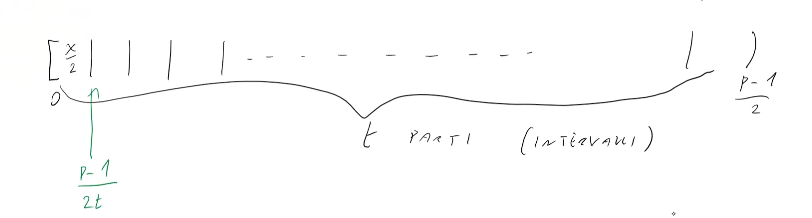
\includegraphics[width=1\textwidth]{images/7.png}
\end{center}
\noindent Supponiamo che $\frac{x}{2}$ sia nel primo intervallo. Qual è la probabilità di trovare un $r$ che vada bene? Se $r$ sta nell'ultimo intervallo, quello che termina con $\frac{p-1}{2}$, effettivamente è possibile che $\frac{x}{2} + r \not< \frac{p-1}{2}$. Ma se $r$ si trova in uno degli altri intervalli, non sarà mai possibile andare oltre $\frac{p-1}{2}$, in quanto il valore di $\frac{x}{2}$ non eccede la dimensione di un intervallo. Quindi la probabilità di trovare un $r$ che vada bene corrisponde alla probabilità di non finire nell'ultimo intervallo. Questa probabilità è:
\begin{align*}
    \frac{t-1}{t}
\end{align*}
\noindent ovvero la probabilità di essere in qualsiasi intervallo tranne l'ultimo. \\

\noindent Prendiamo l'esperimento completo:
\begin{itemize}
    \item Prendi $r$ a caso;
    \item Sia $a$ la PSQR di $yg^{2r}$;
    \item Ritorna $ag^{-r}$.
\end{itemize}
\noindent Scegliamo un $r$ a caso, produciamo il nuovo problema e ne calcoliamo la radice quadrata principale, da quella ricaviamo la risposta al problema originale. 

Qual è la probabilità che la risposta sia corretta? Affinché possiamo avere la garanzia che la risposta sia corretta, ci serve una risposta corretta la problema trasformato ($Pr = \frac{1}{2}k^{-c}$) e sapere di aver scelto una $r$ che soddisfa l'ipotesi del lemma ($Pr = \frac{t-1}{t}$). Quindi la probabilità è:
\begin{align*}
   \left(\frac{t-1}{t}\right) \left(\frac{1}{2}k^{-c}\right)
\end{align*}
\noindent Affinché il trucco di fare tanti esperimenti indipendenti e prendere il maggior numero di risposte corrette come risposta corretta funziona fintanto che la probabilità di dare la risposta corretta sia polinomialmente distante da $\frac{1}{2}$. Quindi la probabilità che avviamo travato deve essere:
\begin{align*}
   \left(\frac{t-1}{t}\right) \left(\frac{1}{2}k^{-c}\right) \ge \frac{1}{2}k^{-2c}
\end{align*}
\noindent Usiamo $k^{-2c}$ in quanto $\frac{t-1}{t}$ rende più piccolo $\left(\frac{1}{2}k^{-c}\right)$, e quindi sarà più vicino a $\frac{1}{2}$. Praticamente la nostra probabilità deve essere maggiore di $\frac{1}{2}$ di un qualsiasi polinomio, solo più piccolo del $k^{-c}$ che avevamo originariamente definito, in quanto sappiamo che $\frac{t-1}{t}$ riduce la nostra probabilità.

Abbiamo quindi imposto che questa grandezza sia sufficientemente distante da $\frac{1}{2}$. Se risolviamo la disequazione in $t$, riusciamo a trovare un limite inferiore al numero di intervalli da usare. Il limite inferiore che ci darà la disequazione sarà un limite polinomiale in $k$. 

Quindi dividendo per una quantità di intervalli che è polinomiale in $k$, riusciamo ad ottenere un sistema tale per cui se $x$ è nel primo intervallo, la probabilità di successo (di fornire una radice quadrata principale di $y$) è polinomialmente distante da $\frac{1}{2}$. Di conseguenza abbiamo un algoritmo polinomiale per calcolare la radice quadrata principale con probabilità di successo esponenzialmente vicina a $1$, grazie al limite di Chernoff.

Abbiamo costruito un algoritmo che con probabilità $\frac{1}{2}$ calcola il logaritmo discreto di un numero a patto che questo logaritmo discreto stia nel primo intervallo. Per portare la probabilità a $1$, basta ripetere l'algoritmo più volte. \\

\noindent Il problema ora è capire come costruire un algoritmo che funzioni su ogni intervallo a partire da uno che funziona con $x$ nel primo intervallo. 

Supponiamo di sapere che $\frac{x}{2}$ si trovi nell'intervallo $i$. L'intervallo i-esimo va da $i \cdot \frac{p-1}{2t}$ a $(i+1) \cdot \frac{p-1}{2t}$, supponendo di numerare gli intervalli con 0, 1, 2, ... . Prendiamo il nostro $y$ e lo moltiplichiamo per $g^{-\frac{p-1}{t}i}$. Cosa stiamo facendo? Sappiamo che $y=g^x$ e che $i \cdot \frac{p-1}{2t} \le \frac{x}{2} < (i+1) \cdot \frac{p-1}{2t}$, quindi se facciamo 
\begin{align*}
    g^{x'} = g^x g^{-\frac{p-1}{t}i}
\end{align*}
\noindent significa che
\begin{align*}
    \frac{x'}{2} = \frac{x - \frac{p-1}{t}i}{2} = \frac{x}{2} - \frac{p-1}{2t}i
\end{align*}

\noindent Con questa moltiplicazione (che diventa una sottrazione sugli esponenti) rimuoviamo il limite sinistro dell'intervallo, spostando il mostro problema dall'intervallo i-esimo al primo. Ci siamo quindi ricondotti al caso che il nostro algoritmo riesce a risolvere. Una volta che il nostro algoritmo avrà risolto il problema, basterà riaggiungere $\frac{p-1}{t}i$ al logaritmo discreto risultate per ottenere la risposta per l'intervallo i-esimo. 

Ci resta solo un problema: come possiamo risolvere il problema se non sappiamo in che intervallo ci troviamo? Basta provarli tutti, tanto sono una quantità polinomiale. Con il primo algoritmo visto siamo in grado di calcolare il logaritmo discreto con probabilità $\frac{1}{2}$ e verificare che sia corretto. Basta ripetere il test per ogni intervallo finché non ci troveremo in quello che rende vera l'ipotesi del lemma. Quindi l'algoritmo che testa una volta ognuna delle ipotesi finché non trova una risposta corretta sappiamo che ci darà la risposta corretta con probabilità almeno $\frac{1}{2}$. Se nessuna delle ipotesi ha dato la risposta corretta, basta ripetere il giro un'altra volta. IN un numero atteso di $2$ tentativi avremo la risposta corretta, il logaritmo discreto di $y$.
\end{proof}

\end{proof}
\end{proof}







































































